% Practice list B (Listas 3-4), Block 3, Question 6: integrative discursive question, symbolic.
% Every closed form, sign, limit and existence/uniqueness claim is verified by practice-L3-L4-check-b3b.py.
\questao{(15 points) Discursive. \emph{Integrative: life-cycle saving $\times$ labor supply $\times$ pension design $\times$ the
interest--growth gap.} Brazil's general regime (INSS) is pay-as-you-go (PAYG), with benefits computed from each worker's
contribution record, while the minimum-wage floor and the non-contributory BPC pay amounts unrelated to it; the 2019 reform
proposal included funded individual accounts (\emph{capitaliza\c{c}\~ao}), dropped in Congress. A household lives two periods: in
period 1 it works $h\in(0,1)$ at the wage $w>0$, in period 2 it is retired. Utility is $u=\ln c_1+\gamma\ln(1-h)+\beta\ln c_2$, with
$\beta\in(0,1)$ and $\gamma>0$. A payroll tax $\tau\in(0,1)$ finances a pension $P$; the budgets are $c_1+a=(1-\tau)wh$ and
$c_2=(1+r)a+P$, with $a$ free in sign. Each generation is $1+n$ times the previous one, wages are constant, $n,r>-1$, prices $(r,w)$ are
taken as given in (a), (b) and (d), and $r>n$ unless stated; write $q\equiv\frac{1+n}{1+r}$. Three designs: \emph{funded},
$P=(1+r)\tau wh$; \emph{Bismarckian PAYG}, $P=(1+n)\tau wh$, linked to the household's own contributions (it internalizes the link);
\emph{Beveridgean PAYG}, a lump sum $P$ that the household takes as given, equal to $(1+n)\tau wh$ in equilibrium.}

\textbf{a)} (3 points) \emph{Funded and Bismarckian designs.} Write each lifetime budget as $c_1+\frac{c_2}{1+r}=\omega wh$ and find
$\omega$. Solve the household problem (both consumptions, and hours $h_F$ and $h_{Bis}$) and compare the two designs.
\resolespaco
\begin{sol}
\passo{lifetime budget (period budgets)}{Substitute $a=(1-\tau)wh-c_1$ into $c_2=(1+r)a+P$ and divide by $1+r$:
$c_1+\frac{c_2}{1+r}=(1-\tau)wh+\frac{P}{1+r}$. Funded: $\frac{P}{1+r}=\tau wh$, so $\omega_F=1$. Bismarck: $\frac{P}{1+r}=q\tau wh$, so
\[\omega=1-\tau+\tau q=1-\frac{\tau(r-n)}{1+r},\]
a weighted average of $1$ and $q$ with weight $\tau$ on $q$: $\omega\in(q,1)$ when $r>n$, and $\omega>0$ always. In both designs $P$ moves
with $h$, so $\omega w$ is what one more hour adds to lifetime resources.}
\passo{FOCs (lifetime budget)}{Add $\omega w(1-h)$ to both sides: $c_1+\frac{c_2}{1+r}+\omega w(1-h)=\omega w\equiv X$, full income. The Lagrangian
$u+\mu\big[X-c_1-\frac{c_2}{1+r}-\omega w(1-h)\big]$ gives $\frac{1}{c_1}=\mu$, $\frac{\beta}{c_2}=\frac{\mu}{1+r}$, $\frac{\gamma}{1-h}=\mu\,\omega w$, where $\mu$ is the marginal
utility of lifetime wealth; $u$ is strictly concave and the budget linear, so the FOCs give the unique optimum. Spending on each good
is its weight over $\mu$; summing, $X=(1+\beta+\gamma)/\mu$.}
\passo{solution (FOCs and $X=\omega w$)}{
\[c_1=\frac{\omega w}{1+\beta+\gamma},\qquad c_2=\frac{\beta(1+r)\,\omega w}{1+\beta+\gamma},\qquad h=\frac{1+\beta}{1+\beta+\gamma}.\]
Hours depend on neither $\omega$ nor $w$: full income and the price of leisure are both proportional to $\omega w$, so with log utility
the income and substitution effects of $\omega$ cancel.}
\passo{comparison}{$h_{Bis}=h_F$ and $c_t^{Bis}=\omega\,c_t^{F}$ for $t=1,2$. A Bismarckian system is a funded one whose contributions earn
the growth rate $n$ instead of $r$: with $r>n$ it is a pure wealth loss of $1-\omega$ of lifetime income, with no distortion.}
\intuicao{The link between contributions and benefits keeps the leisure margin intact: the household treats the tax as saving at
return $n$, so only its lifetime wealth changes.}
\refbib{Kurlat (2020), \S6.2 (two-period consumption) and \S7.2, \S7.4 (labor--leisure choice, jointly with saving); Romer (2012),
Problem 2.17 (social security in the Diamond model).}
\rubrica{
\item Lifetime budget and $\omega$, with $\omega\in(q,1)$: 1 pt.
\item FOCs, full income and the three closed forms: 1.5 pts. Hours quoted from the static model instead of derived: max.\ a third of the item.
\item Independence of hours from $\omega$ and the scaling by $\omega$: 0.5 pt.
}
\end{sol}

\textbf{b)} (3 points) \emph{Beveridgean design.} Find equilibrium hours $h_{Bev}$, compare them with $h_F$, explain the mechanism, and draw
hours against $\tau\in(0,1)$ for the three designs.
\resolespaco
\begin{sol}
\passo{household problem ($P$ given)}{The lifetime budget is $c_1+\frac{c_2}{1+r}=(1-\tau)wh+\frac{P}{1+r}$: the price of leisure is now $(1-\tau)w$ and full
income $X=(1-\tau)w+\frac{P}{1+r}$. The FOCs of (a), with $\omega w$ replaced by $(1-\tau)w$, give $(1-\tau)w(1-h)=\frac{\gamma X}{1+\beta+\gamma}$.}
\passo{equilibrium (pension budget, after the FOC)}{Impose $\frac{P}{1+r}=q\tau wh$, so $X=(1-\tau)w+q\tau wh$:
\[(1+\beta+\gamma)(1-\tau)(1-h)=\gamma(1-\tau)+\gamma q\tau h\ \Longrightarrow\ h_{Bev}=\frac{(1+\beta)(1-\tau)}{(1+\beta)(1-\tau)+\gamma\omega},\]
using $1-\tau+q\tau=\omega$.}
\passo{comparison}{With $x\equiv\frac{1-\tau}{\omega}$, $h_{Bev}=\frac{(1+\beta)x}{(1+\beta)x+\gamma}$, strictly increasing in $x$, and $h_F$ is its value at $x=1$. Since
$\omega-(1-\tau)=q\tau>0$, $x<1$ and $h_{Bev}<h_F$ for every $r$ and $n$, including $r\le n$. As $\tau\to1$, $h_{Bev}\to0$.}
\passo{the wedge}{In equilibrium an hour adds $\omega w$ to lifetime resources (budget above), but the household prices leisure at
$(1-\tau)w$: it sees the tax and not the return $q\tau w$ that comes back as a pension. Relative to Bismarck, Beveridge taxes the
marginal hour at the rate $q\tau/\omega$ and rebates the revenue lump sum (Prescott's tax--transfer experiment): the rebate offsets the
income effect, and the substitution effect lowers hours.}
\begin{center}
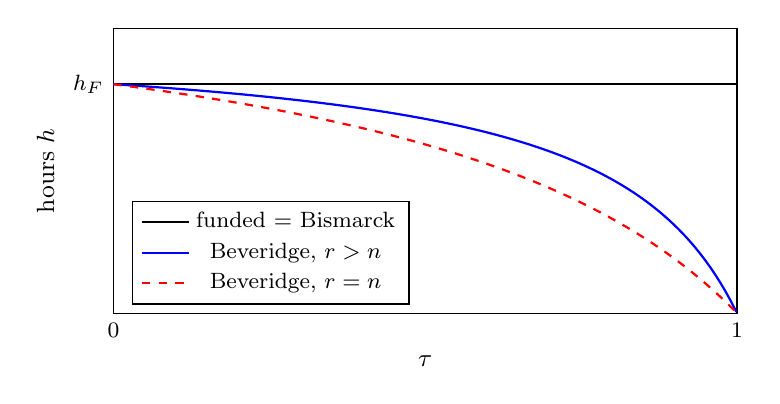
\begin{tikzpicture}
\begin{axis}[width=9.5cm,height=5.2cm,xmin=0,xmax=1,ymin=0,ymax=0.8,xlabel={$\tau$},ylabel={hours $h$},
  xtick={0,1},xticklabels={$0$,$1$},ytick={0.642857},yticklabels={$h_F$},legend pos=south west,
  legend style={font=\footnotesize},tick label style={font=\footnotesize},label style={font=\small}]
\addplot[thick,black,domain=0:1,samples=2]{1.8/2.8};
\addplot[thick,blue,domain=0:0.999,samples=120]{1.8*(1-x)/(1.8*(1-x)+(1-x+0.5*x))};
\addplot[thick,red,dashed,domain=0:0.999,samples=120]{1.8*(1-x)/(1.8*(1-x)+1)};
\legend{funded $=$ Bismarck,{Beveridge, $r>n$},{Beveridge, $r=n$}}
\end{axis}
\end{tikzpicture}
\end{center}
\intuicao{Beveridge breaks the link between the marginal contribution and the benefit, so the payroll tax becomes a labor tax; the
curve for $r=n$ lies lower because a pension worth more in present value returns a larger share of each contribution as a lump
sum that the household does not link to its hours (the wedge $q\tau/\omega$ rises with $q$).}
\refbib{Kurlat (2020), \S7.2--7.3 (taxes and social security as Prescott's explanation of hours) and Exercise 7.5.}
\rubrica{
\item FOC with $P$ taken as given: 0.5 pt.
\item $h_{Bev}$ with the pension substituted after the FOC: 1 pt. Substituting before the FOC (the Bismarck problem): max.\ half of the item.
\item Proof of $h_{Bev}<h_F$ and the wedge: 0.5 pt.
\item Graph (scored separately): axes and labels; flat line at $h_F$ for funded and Bismarck; Beveridge curve falling from $h_F$ at
$\tau=0$ towards $0$ as $\tau\to1$: 1 pt.
}
\end{sol}

\textbf{c)} (3 points) \emph{Saving and capital.} Find private saving per unit of wage income, $a/(wh)$, in both PAYG designs, and the
national saving rates $s_F$, $s_{Bis}$ and $s_{Bev}$ (private saving plus pension assets, per unit of wage income); rank them. If these
are the saving rates of a Cobb--Douglas Solow economy with capital share $\alpha\in(0,1)$, the same $n$, technology growth $g$ and
depreciation $\delta$ ($\delta+n+g>0$), by what factor does each PAYG design change steady-state output per effective worker relative to
the funded design?
\resolespaco
\begin{sol}
\passo{full income per unit of wage income}{In both PAYG designs $c_1=\frac{X}{1+\beta+\gamma}$ (FOCs). Bismarck: $X=\omega w$ and
$wh=\frac{(1+\beta)w}{1+\beta+\gamma}$. Beveridge: the hours equation of (b) gives $\frac{1-\tau}{h_{Bev}}=(1-\tau)+\frac{\gamma\omega}{1+\beta}$, so
$\frac{X}{wh}=\frac{1-\tau}{h_{Bev}}+q\tau=\omega\big(1+\frac{\gamma}{1+\beta}\big)$. In both designs,
\[\frac{X}{wh}=\frac{\omega(1+\beta+\gamma)}{1+\beta}\ \Longrightarrow\ \frac{c_1}{wh}=\frac{\omega}{1+\beta},\qquad\frac{a}{wh}=(1-\tau)-\frac{\omega}{1+\beta}.\]}
\passo{national saving rates}{PAYG holds no assets, so national saving is the private saving above, the same in both designs:
$s_{Bis}=s_{Bev}=(1-\tau)-\frac{\omega}{1+\beta}=\frac{\beta-\tau(\beta+q)}{1+\beta}\equiv s_{PAYG}$.
Funded: $c_1=\frac{wh}{1+\beta}$, private saving is $\frac{a_F}{wh}=\frac{\beta}{1+\beta}-\tau$ (negative if $\tau>\frac{\beta}{1+\beta}$: the household borrows against
its pension), and adding the fund's assets $\tau$ gives $s_F=\frac{\beta}{1+\beta}$, independent of $\tau$.}
\passo{ranking}{$s_F-s_{PAYG}=\frac{\tau(\beta+q)}{1+\beta}=\tau-\frac{1-\omega}{1+\beta}>0$: PAYG removes the fund ($-\tau$), and the household, poorer by
$1-\omega$, cuts $c_1$ by $\frac{1-\omega}{1+\beta}$ and saves that much more, a partial offset.}
\passo{Solow (Kurlat ch.~4)}{Per efficiency unit of labor, $\tilde y=\tilde k^{\alpha}$ and the steady state solves $s\,\tilde y=(\delta+n+g)\tilde k$, so
$\tilde y^*=\big(\frac{s}{\delta+n+g}\big)^{\frac{\alpha}{1-\alpha}}$; measuring saving out of output, $(1-\alpha)s$, changes nothing below. The common
terms cancel, and both PAYG designs give the same factor ($j=Bis,Bev$):
\[\frac{\tilde y^*_{j}}{\tilde y^*_F}=\Big(\frac{s_{PAYG}}{s_F}\Big)^{\frac{\alpha}{1-\alpha}}=\Big[1-\tau\Big(1+\frac{q}{\beta}\Big)\Big]^{\frac{\alpha}{1-\alpha}}\in(0,1)
\qquad\text{for }\tau<\frac{\beta}{\beta+q},\]
the condition for positive PAYG saving. Per worker, Beveridge loses a further factor $h_{Bev}/h_F$: output per worker is
$A\,h\,\tilde y$ ($A$: labor-augmenting technology).}
\intuicao{A funded system is forced saving that the household undoes one for one, so it is neutral for capital; a PAYG system pays
the old out of the young's contributions, which never become capital. Both PAYG designs save the same share because they face the
same interest rate and the same equilibrium lifetime resources per hour, $\omega wh$, which the Euler equation splits in the same way.}
\refbib{Kurlat (2020), \S4.2 and \S4.5 (steady state per efficiency unit of labor), \S6.2 (Euler equation); Romer (2012), Problem 2.17.}
\rubrica{
\item $X/(wh)$ in both designs and $a/(wh)$: 1 pt. Shown for one design only: 0.5 pt.
\item $s_F$, $s_{Bis}=s_{Bev}$ and the ranking, proved: 1 pt.
\item Solow ratio with the positivity condition: 1 pt. Ratio not linked to the saving rates derived here (answered inside one model): max.\ half of the item.
}
\end{sol}

\textbf{d)} (3 points) \emph{Welfare.} At given prices, measure each PAYG design by its consumption-equivalent loss $\lambda$ relative to
funded: the share of funded consumption in both periods, at funded hours, whose loss leaves the household as well off as under the
PAYG design. Find $\lambda_{Bis}$ and $\lambda_{Bev}$ in closed form, rank the three designs when $r>n$ (the two PAYG designs by a
revealed-preference argument), and determine what changes when $r=n$ and when $r<n$.
\resolespaco
\begin{sol}
\passo{definition}{Scaling both consumptions by $1-\lambda$ changes utility by $(1+\beta)\ln(1-\lambda)$, so $\lambda_j$ solves
$U_F+(1+\beta)\ln(1-\lambda_j)=U_j$.}
\passo{Bismarck (from (a))}{Same hours, consumptions scaled by $\omega$: $U_{Bis}=U_F+(1+\beta)\ln\omega$, so $\lambda_{Bis}=1-\omega=\frac{\tau(r-n)}{1+r}$.}
\passo{Beveridge (from (b), (c))}{$c_1=\frac{\omega wh}{1+\beta}$ in both PAYG designs and $\frac{wh}{1+\beta}$ when funded, and $c_2=\beta(1+r)c_1$ in all
three, so $c_t^{Bev}/c_t^F=\omega h_{Bev}/h_F$. With $\frac{h_{Bev}}{h_F}=\frac{(1+\beta+\gamma)x}{(1+\beta)x+\gamma}$, $\frac{1-h_{Bev}}{1-h_F}=\frac{1+\beta+\gamma}{(1+\beta)x+\gamma}$, $\omega x=1-\tau$
and $\rho\equiv\frac{1+\beta+\gamma}{1+\beta}>1$:
\[1-\lambda_{Bev}=\frac{\omega h_{Bev}}{h_F}\Big(\frac{1-h_{Bev}}{1-h_F}\Big)^{\frac{\gamma}{1+\beta}}=(1-\tau)\Big[\frac{(1+\beta+\gamma)\,\omega}{(1+\beta)(1-\tau)+\gamma\omega}\Big]^{\rho}.\]}
\passo{ranking by revealed preference}{In equilibrium the Beveridge allocation satisfies $c_1+\frac{c_2}{1+r}=(1-\tau)wh_{Bev}+q\tau wh_{Bev}=\omega wh_{Bev}$,
so it is affordable under Bismarck. The Bismarck choice is the unique maximizer of the strictly concave $u$ on that convex set, and
$h_{Bev}\neq h_{Bis}$ by (b), so $U_{Bev}<U_{Bis}$: $\lambda_{Bev}>\lambda_{Bis}$. With $r>n$, $\omega<1$ and $U_F>U_{Bis}>U_{Bev}$.}
\passo{$r=n$}{$q=\omega=1$: $\lambda_{Bis}=0$, Bismarck replicates funded. Beveridge still distorts hours ($x=1-\tau<1$), and by the
previous step $\lambda_{Bev}=1-(1-\tau)\big[\frac{1+\beta+\gamma}{(1+\beta)(1-\tau)+\gamma}\big]^{\rho}>0$.}
\passo{$r<n$ (dynamic inefficiency)}{PAYG now pays $n>r$: $\lambda_{Bis}=-\frac{\tau(n-r)}{1+r}<0$, Bismarck beats funded. For Beveridge, with
$b\equiv1-\frac{\gamma q}{1+\beta+\gamma}$ (so that $(1+\beta)(1-\tau)+\gamma\omega=(1+\beta+\gamma)(1-b\tau)$), let
$L(\tau)\equiv\ln(1-\lambda_{Bev})=\ln(1-\tau)+\rho\ln\omega-\rho\ln(1-b\tau)$. Then $L(0)=0$ and
\[L'(\tau)=\frac{q}{\omega(1-b\tau)}-\frac{1}{1-\tau}=\frac{N(\tau)}{(1-\tau)\,\omega\,(1-b\tau)},\qquad N(\tau)\equiv q(1-\tau)-\omega(1-b\tau).\]
$N$ has degree at most 2, $N(0)=q-1>0$ and $N(1)=-\frac{\gamma q^2}{1+\beta+\gamma}<0$, so it has exactly one root $\tau_p\in(0,1)$: $L$ rises on
$(0,\tau_p)$ and falls on $(\tau_p,1)$, with $L\to-\infty$ as $\tau\to1$. Hence there is a unique $\bar\tau\in(\tau_p,1)$, with no closed form, such that
Beveridge beats funded if and only if $\tau<\bar\tau$.}
\intuicao{Bismarck costs only the return gap $1-\omega$, which changes sign with $r-n$. Beveridge adds an hours distortion that survives
at $r=n$; with $r<n$ a small Beveridge system still gains, because its return gain is first order in $\tau$ ($L'(0)=q-1$) while the
distortion is second order (see (e)).}
\refbib{Romer (2012), \S2.11 (dynamic inefficiency) and Problem 2.17; Kurlat (2020), \S4.3 (golden rule).}
\rubrica{
\item Definition of $\lambda$ and $\lambda_{Bis}$: 0.5 pt.
\item $\lambda_{Bev}$ in closed form: 1 pt. Quoted instead of derived: max.\ a third of the item.
\item Revealed-preference ranking (affordability, uniqueness, $h_{Bev}\neq h_{Bis}$): 0.5 pt. Ranking asserted or read off numbers: 0 for that line.
\item $r=n$, and $r<n$ with $\bar\tau$ proved to exist and be unique: 1 pt. ``PAYG beats funded'' claimed for Beveridge without the condition: 0 for that line.
}
\end{sol}

\textbf{e)} (3 points) \emph{Parameter analysis.} Sign the effects of $r$, $n$ and $\tau$ on $\omega$, $h_{Bev}$, $s_{Bis}$, $s_{Bev}$, the two Solow
output ratios of (c), $\lambda_{Bis}$ and $\lambda_{Bev}$; prove each sign and collect the signs in a table; find the limits $\tau\to0$ (with the order
in $\tau$ of $\lambda_{Bev}-\lambda_{Bis}$) and $r\to n$, and read the results.
\resolespaco
\begin{sol}
\passo{$\omega$ and $\lambda_{Bis}$}{From $\omega=1-\tau+\tau q$: $\frac{\partial\omega}{\partial r}=-\frac{\tau(1+n)}{(1+r)^2}<0$, $\frac{\partial\omega}{\partial n}=\frac{\tau}{1+r}>0$,
$\frac{\partial\omega}{\partial\tau}=q-1=-\frac{r-n}{1+r}$, with the sign of $n-r$. $\lambda_{Bis}=1-\omega$ has the opposite signs.}
\passo{$h_{Bev}$}{$\frac{\partial h_{Bev}}{\partial x}=\frac{(1+\beta)\gamma}{[(1+\beta)x+\gamma]^2}>0$, and from $x=\frac{1-\tau}{\omega}$: $\frac{dx}{d\tau}=\frac{-\omega-(1-\tau)(q-1)}{\omega^2}=-\frac{q}{\omega^2}<0$,
$\frac{\partial x}{\partial r}=-\frac{x}{\omega}\frac{\partial\omega}{\partial r}>0$, $\frac{\partial x}{\partial n}=-\frac{x}{\omega}\frac{\partial\omega}{\partial n}<0$. So $h_{Bev}$ falls with $\tau$ for any $(r,n)$, rises with $r$ and falls with $n$.}
\passo{saving and output}{From $s_{Bis}=s_{Bev}=s_{PAYG}=\frac{\beta-\tau(\beta+q)}{1+\beta}$ (c): $\frac{\partial s_{PAYG}}{\partial r}=\frac{\tau(1+n)}{(1+\beta)(1+r)^2}>0$,
$\frac{\partial s_{PAYG}}{\partial n}=-\frac{\tau}{(1+\beta)(1+r)}<0$, $\frac{\partial s_{PAYG}}{\partial\tau}=-\frac{\beta+q}{1+\beta}<0$. Since $s_F$ is constant and $z\mapsto z^{\alpha/(1-\alpha)}$ is
increasing, both output ratios have the same signs.}
\passo{$\lambda_{Bev}$ in $r$ and $n$}{At fixed $\tau$, $r$ and $n$ enter $1-\lambda_{Bev}$ only through $\omega$, and
\[\frac{\partial\ln(1-\lambda_{Bev})}{\partial\omega}=\frac{\rho}{\omega}-\frac{\rho\gamma}{(1+\beta)(1-\tau)+\gamma\omega}=\frac{\rho(1+\beta)(1-\tau)}{\omega\,[(1+\beta)(1-\tau)+\gamma\omega]}>0,\]
so $\lambda_{Bev}$ rises with $r$ and falls with $n$, like $\lambda_{Bis}$.}
\passo{$\lambda_{Bev}$ in $\tau$}{Write $1-\lambda_{Bev}=\omega\,e^{\varphi(x)}$ with $\varphi(x)\equiv\ln x+\rho\ln\frac{1+\beta+\gamma}{(1+\beta)x+\gamma}$: $\varphi(1)=0$ and
$\varphi'(x)=\frac{\gamma(1-x)}{x[(1+\beta)x+\gamma]}>0$ on $(0,1)$, so $e^{\varphi(x)}=\frac{1-\lambda_{Bev}}{1-\lambda_{Bis}}<1$, the analytic twin of (d). Then
$L'(\tau)=\frac{q-1}{\omega}-\varphi'(x)\frac{q}{\omega^2}<0$ if $r\ge n$: $\lambda_{Bev}$ rises with $\tau$. If $r<n$, $\lambda_{Bev}$ falls on $(0,\tau_p)$ and rises on $(\tau_p,1)$, by (d).}
\begin{center}
\begin{tabular}{lccc}
\toprule
 & $r$ & $n$ & $\tau$ \\
\midrule
$\omega$ & $-$ & $+$ & sign of $n-r$ \\
$h_{Bev}$ & $+$ & $-$ & $-$ \\
$s_{Bis}=s_{Bev}$, both output ratios & $+$ & $-$ & $-$ \\
$\lambda_{Bis}$ & $+$ & $-$ & sign of $r-n$ \\
$\lambda_{Bev}$ & $+$ & $-$ & $+$ if $r\ge n$; $-$ then $+$ (at $\tau_p$) if $r<n$ \\
$h_F=h_{Bis}$, $s_F$ & $0$ & $0$ & $0$ \\
\bottomrule
\end{tabular}
\end{center}
\passo{limit $\tau\to0$}{$\omega,x\to1$: $h_{Bev}\to h_F$, $s_{PAYG}\to s_F$, both output ratios $\to1$, and $\lambda_{Bis},\lambda_{Bev}\to0$. $\lambda_{Bis}=(1-q)\tau$ is first order,
while $\lambda_{Bev}-\lambda_{Bis}=\omega\big(1-e^{\varphi(x)}\big)$, with $\varphi(1)=\varphi'(1)=0$, $\varphi''(1)=-\frac{\gamma}{1+\beta+\gamma}$ and $x-1=-\frac{q\tau}{\omega}$, gives
\[\lambda_{Bev}-\lambda_{Bis}=\frac12\,\frac{\gamma}{1+\beta+\gamma}\,(q\tau)^2+O(\tau^3):\]
a Harberger triangle, one half times the leisure share of full income times the squared wedge $q\tau$.}
\passo{limit $r\to n$}{$q,\omega\to1$: $\lambda_{Bis}\to0$, but $h_{Bev}\to\frac{(1+\beta)(1-\tau)}{(1+\beta)(1-\tau)+\gamma}<h_F$, $\lambda_{Bev}$ stays positive by (d), and $s_{PAYG}\to s_F-\tau$:
at $r=n$ Bismarck is harmless to the household and still lowers saving by the whole contribution.}
\intuicao{The interest--growth gap prices the first-order cost of PAYG, $1-\omega=\tau(r-n)/(1+r)$; the benefit--contribution link
decides the second-order cost in hours, which only Beveridge pays and whose leading term grows with $\gamma$ and $\tau$. A higher $r$
makes PAYG costlier but, by lowering the present value of the pension, raises Beveridge hours and PAYG saving. Saving is lower
under PAYG for every $(r,n)$, so the capital cost does not vanish where the household's cost does.}
\refbib{Kurlat (2020), \S4.3 and \S7.3; Romer (2012), \S2.11.}
\rubrica{
\item Signs of $\omega$, $h_{Bev}$, $s_{Bis}=s_{Bev}$, the output ratios and $\lambda_{Bis}$, each proved: 1 pt.
\item Signs of $\lambda_{Bev}$ in $r$, $n$, and in $\tau$ by case, proved: 0.5 pt.
\item Table of signs: 0.5 pt. Limits, including the second-order term: 0.5 pt.
\item Reading: 0.5 pt. Signs listed without proofs or without the reading: max.\ half of the item.
}
\end{sol}
